\documentclass{report}
\author{Samiran Das, 24B1270\\
Mentor \- Revanth Manepalli}
\usepackage{amsmath}
\usepackage{graphicx}
\title{SoS '25 Mid-term Report\\
Control Systems}

\begin{document}

\maketitle

\chapter{Introduction}

\section{Definition:}
A Control System consists of subsytem and processes or plants assembled 
in such a way that we can obtain a desired performance given a specific input.

\begin{figure}[htbp]
    \centering
    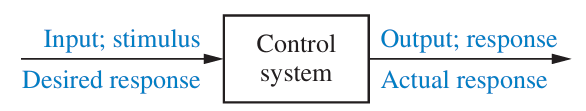
\includegraphics[scale=0.5]{images/cs_simple_bd.png}
    \caption{Simplified description of a Control System.}
\end{figure}

\section{Applications:}
Control systems make moving large equipments with insane precision possible.
An elevator reaching precisely leveled and alligned with the floor we input,
pointing huge antennas towards the farthest reaches of the universe precisely
to pick up faint radio signals are some examples of what we can achieve with well designed Control systems.
\par
We design control systems for four primary reasons:
\begin{itemize}
    \item \textbf{Power Amplification:} For example, the movement of a heavy piece of equipment is
    controlled by low-power input of a potentiometer or similar sensors and a large amount of power
    is required for output. A well designed control system can produce the required power amplification
    or power gain for it.
    \item \textbf{Remote Control:} Control system plays a great role in remote control of robotics equipment
    which can compensate for human disabilities in hazardoues environment.
    \item \textbf{Convenience of input form:} Control system can also be used for various form of inputs for convenience.
    For example, in a temperature control system, the input is a position on a thermostat. The output is heat. Thus, a convenient
    position input yields a desired thermal output.
    \item \textbf{Compensation for disturbances:} One more advantage is that a well designed control system can compensate disturbances
    by measuring noises in input signal and subsequently correcting that in the output.
\end{itemize}

\section{Open vs. Closed loop Control Systems:}

\begin{figure}[htbp]
    \centering
    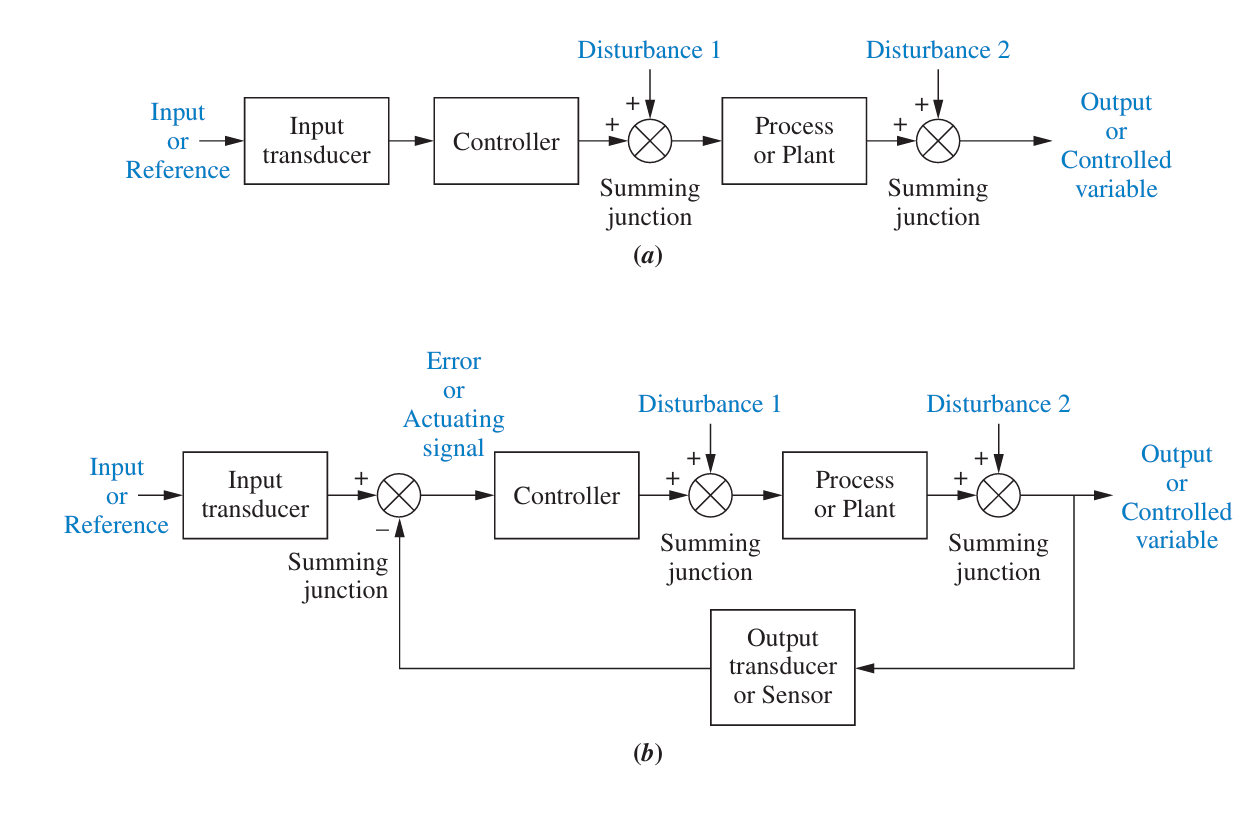
\includegraphics[scale=0.3]{images/Open&Closed_loop_control.png}
    \caption{System configuration: (a) Open-loop, (b) Closed-loop}
\end{figure}
\par
The block diagram of an generic \textit{open-loop system} is shown in figure 1.2 (a). It starts with the \textit{input transducer}, which converts
the form of input used by the controller. The \textit{input} is also sometimes called \textit{reference}, while the \textit{output} can be called
\textit{controlled variable}. In the system \textit{disturbances} are also added to \textit{controller} and \textit{process} output via \textit{summing juctions},
which outputs the sum of input signals using associated signs.
\\
\par
The characteristic that distinguishes \textit{open-loop system} from the another is that it cannot compensate for the disturbances added to the controller's driving-signal.
Thus, the output of \textit{open-loop system} is not only affected by the controller's command, but also disturbances at the output.
\\
\par
A good example of such system is a washing machine. Depending upon the input selected it only washes and spins for some dedicated time. But, the washing action depends on
various factors like hardness of water, temperature, detergent used etc which contributes to external disturbances and the clothes may not be washed as clean as expected by the user.
These disturbances cannot be compensated by the controller of the washing machine.
\\
\par
These issues can be mitigated by a \textit{Closed-loop or Feedback control system}. The generithwc architecture of this system is shown in figure 1.2 (b). The difference here is an
output transducer placed in the output which creates a \textit{feedback path} coverting to the form used by the controller to controller itself. The first summing junction adds
the input signal algebriacally to the output signal coming via the \textit{feedback path}. The output signal is substracted from the input signal. The resulting signal is called
actuating signal. However, in systems where the input and the output transducer have \textit{unity gain}, the actuating signal is just difference between output and input signal. In this
case the actuating signal is also called error.
\\
\par
These \textit{closed-loop} systems can compensate for disturbances by measuring the output signal, feeding back through feedback path and comparing with input signal in the summing junction.
If there is any difference between the two signal, the actuating signal drives the plant to make a correction for the error. If there's no difference, the plant doesn't give any driving signal
as the system has already reached the desired output.
\\
\par
\textit{Closed-loop} systems always have greater accuracy than \textit{open-loop} systems and the advantages of being sensitive to noises, disturbances and changes in the environment.
Transient response and steady-state errors are always controlled by a \textit{closed-loop system} more conveniently and with greater flexibility often with minimal changes.

\chapter{Time vs. Frequency Domain Perspectives}
\section{Time Domain:}
\par
In the time domain, the analytical approach we take is to observe the change in the system's output over \textit{time} in response to inputs like \textit{steps} or \textit{impulses}. This analytical approach is rooted
            in solving \textit{differential equations} and examinig the performance metrics such as \textit{rise time, overshoot, settling time} and \textit{steady-state error}.
\\
\par
The great thing about this perspective is that it highlights \textit{transient behaviour}, detecting overshoot, damping effects and how quickly the system reaches stability. It has great compatibility
for \textit{non-linear} and \textit{multi-variable dynamics} while incorporating some powerfull methods like \textit{State-Space} representations. It's sometimes very useful for understanding how an actual real-life
system responds in time.
\\
\par
While being useful in some cases, it also has some disadvantages. It requires complex mathematical analysis often working with higher-order differential equations,
which are difficult to solve analytically and often require numerical method or computational approach. As the name suggest, it always works with time-dependent behaviours,
which limits insight to \textit{frequency-dependent} behaviours, making it less straightforward to assess aspects like resonance, bandwidth or noise implications. It can also make
the controller design more challanging as it often lacks the systematic loop-shaping capabillities that frequency-domain tools like Bode plots and
Nyquist diagrams offers.

\section{Frequency Domain:}
This approach transforms time-dependent differential equations into \textit{frequency domain} using \textit{Laplace} or \textit{Fourier} transforms. In this approach, we focus on how the system responds to different frequencies of inputs
signals (sinusoids), analyzing \textit{gain} and \textit{phase} relationships over the spectrum.
\\
\par
In this perspective, it becomes quite easy to study the \textit{stability margins}, \textit{resonance} and \textit{bandwidth}. Here, the \textit{phase} and \textit{gain} margins become apparant through
\textit{Bode plots} and \textit{Nyquist diagrams} revealing risks of \textit{oscillations} and \textit{instability}. We can see which frequencies are amplified or attenuated which is critical for control and
robustness design. And the best part, it transforms differential equations into \textit{algebriac} equations, making controller design easier and simpler.
\\
\par
Even with these advantages, this perspective suffers from various imcopatibility and reliability issues as it's limited to only linear, time-invariant (LTI) systems. So, non-linear and time-varying dynamics cannot be accurately modelled in this
perspective. Here, due to loss of \textit{time-dependent} information, this perspective makes some event like sudden spikes or timing criticalities less detectable. Sometimes it also demands high computational power in constructing high-resolution
Bode plots or Nyquist diagrams, specifically at extreme frequency ranges as it's often computationally intensive and sensitive to modelling assumptions.
\\
\par
Frequency domain analysis excels at \textit{stability} and \textit{robustness}, with ability to traslate complex dynamics into interpretable \textit{gain} and \textit{phase} relationships. However, it's restricted only to \textit{LTI frameworks},
can obscure transient event details, and often requires careful modelling and sufficient computational effort to be effective.

\chapter{Linear, Time-Invariant (LTI) Systems}

\section{LTI (Linear, Time-invariant) Systems:}
\subsection{Definition:}
A \textit{Linear, Time-invariant system} is a class of dynamic systems characterised by two basic and fundamental prooerties:
\begin{itemize}
    \item \textit{Linearity:} This system obeys the principle of superposition, which includes
    \begin{itemize}
        \item Additivity: if $y_1(t)=f(x_1(t))$ (i.e $y_1$ output corresponds to $x_1$ input) and $y_2(t)=f(x_2(t))$, then $y_1(t)+y_2(t)=f(x_1(t)+x_2(t))$.
        \item Homogeniety: if $y(t)=f(x(t))$, then $ky(t)=f(kx(t))$.
    \end{itemize}
    \item \textit{Time invariance:} The system's behavior does not change over time. If an input produces a certain output, delaying the input by a time shift will delay the output by the same amount, without altering its shape.
    \\
    \par
    That means $y(t)=f(x(t))$ can be altered to $y(t-\tau)=f(x(t-\tau))$
\end{itemize}

\subsection{Features and Mathematical Representations}
\begin{itemize}
    \item \textbf{Differential or Difference Equations}: LTI systems are typically described using linear constant-coefficient differential equations (continuous-time) or difference equations (discrete-time).
    \item \textbf{Impulse Response:} The output of an LTI system to a Dirac delta function input is known as the impulse response, which completely characterizes the system.
    \item \textbf{Convolutional operation:} The output of an LTI system to any arbitrary input can be computed as the convolution of the input signal with the impulse response.
    \\
    \begin{equation}
        y(t) = (x * h)(t) = \int_{-\infty}^{\infty} x(\tau) h(t - \tau) d\tau
    \end{equation}
    \item \textbf{Tranfer function:} In the frequency (Laplace or Z) domain, LTI systems can be represented as transfer functions, which express the output/input ratio as a rational function of $s$ (a complex frequency variable)
\end{itemize}

\subsection{Advantages of LTI Systems:}
\begin{itemize}
    \item \textbf{Predictability:} Due to their mathematical regularity, LTI systems are easier to analyze and design.
    \item \textbf{Transfrom simplifiction:} Tools like the Laplace and Fourier transforms convert complex differential equations into simple algebraic forms.
    \item \textbf{Control and Signal Processing Applications:} LTI models form the foundation for most classical control theory and digital filter design.
\end{itemize}

\subsection{Limitations:}
While being so useful, easier to work with and featureful, it also suffers from some limitations such as,
\begin{itemize}
    \item \textbf{Not Universally Applicable}: Many real-world systems (e.g., systems with saturation, hysteresis, or time-varying parameters) are nonlinear or time-variant and cannot be perfectly modeled as LTI.
    \item \textbf{Idealizations}: Time invariance assumes a perfectly stable environment, which may not always be true in practical scenarios like sensor drift or actuator wear.
\end{itemize}

\subsection{Summary:}
LTI systems serve as the backbone of classical control and signal processing. Their rich theoretical properties make them easy to understand and powerful to use, enabling us to build accurate models,
design robust controllers, and apply analytical tools with confidence. While idealized, they often serve as a first approximation before addressing more complex, real-world nonlinearity or time variance.

\chapter{Transfer Functions}

\section{Definition:}
A transfer function is a mathematical representation of the relationship between the input and output of a \textit{linear, time-invariant (LTI) system} in the frequency (Laplace) domain. It is defined as the ratio of the Laplace transform of the output to that of the input, under zero initial conditions:

\begin{equation}
    G(s) = \frac{Y(s)}{X(s)}
\end{equation}
where:

$G(s)$ is the transfer function

$X(s)$ is the Laplace transform of the input signal

$Y(s)$ is the Laplace transform of the output signal

$s$ is the complex frequency variable 

\par
A typical transfer function has the form:

\begin{equation}
    G(s) = \frac{b_m s^m + \dots + b_1 s + b_0}{a_n s^n + \dots + a_1 s + a_0}
\end{equation}
\\
\par
This rational function relates the system dynamics using:

\begin{itemize}
    \item Numerator coefficients that influence zeros of the system
    \item Denominator coefficients that define the poles (roots of the characteristic equation)
\end{itemize}

\section{Example:}
Let us take an example of an RLC network as shown in the below figure 4.1. We will find the transfer function relating the capacitor voltage $V_C(s)$,to the input voltage $V(s)$.
\begin{figure}[htbp]
    \centering
    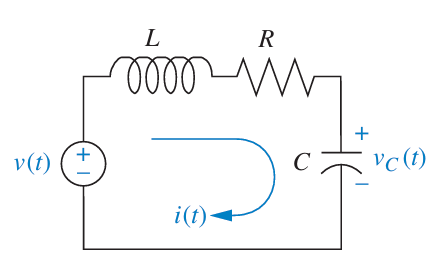
\includegraphics[scale=0.5]{images/RLC_Network.png}
    \caption{RLC network}
\end{figure}
\\
\par
We'll treat the capacitor voltage as output and supplied voltage as input. Summing the voltages around the loop, assuming zero initial conditions,
yields the following equation for this network as
\begin{equation}
    L\frac{di(t)}{dt}+Ri(t)+\frac{1}{C}\int_{0}^{t}i(\tau)d\tau=v(t)
\end{equation}
Changing variable from $i(t)$ to $q(t)$ using $i(t)=\frac{d}{dt}q(t)$,
\begin{equation}
    L\frac{d^2q(t)}{dt^2}+R\frac{d}{dt}q(t)+\frac{1}{C}q(t)=v(t)
\end{equation}
Taking the voltage charge relation $q(t=Cv_C(t))$
\begin{equation}
    LC\frac{d^2v_C(t)}{dt^2}+RC\frac{d}{dt}v_C(t)+v_c(t)=v(t)
\end{equation}
Taking the Laplace transform assuming zero initial conditions, rearranging terms, and simplifying yields
\begin{equation}
    (LCs^2+RCs+1)V_C(s)=V(s)
\end{equation}
Solving for transfer function $G(s)=\frac{V_C(s)}{V(s)}$ we obtain,
\begin{equation}
    G(s)=\frac{\frac{1}{LC}}{s^2+\frac{R}{L}s+\frac{1}{LC}}
\end{equation}


\section{Advantages:}
\begin{itemize}
    \item \textbf{Simplifies Differential Equations}: Converts time-domain differential equations into algebraic expressions that are easier to manipulate.
    \item \textbf{Enables Frequency Domain Analysis}: Facilitates use of Bode plots, Nyquist plots, and root locus techniques.
    \item \textbf{Modularity}: Systems can be modeled as blocks (transfer functions), and interconnected using simple algebra (series, parallel, feedback loops).
    \item \textbf{Facilitates Control Design}: Supports stability analysis, performance tuning, and feedback controller design in both academic and industrial settings.
\end{itemize}

\section{Limitations:}
\begin{itemize}
    \item \textbf{Applicable Only to LTI Systems}: Cannot directly handle nonlinear or time-varying systems.
    \item \textbf{Assumes Zero Initial Conditions}: Initial state responses are ignored unless specifically modeled separately.
    \item \textbf{No Internal State Insight}: Transfer functions capture input-output behavior, but do not provide information about internal system states—unlike state-space models.
\end{itemize}

\section{Summary:}
Transfer functions offer a compact and powerful way to describe and analyze dynamic systems. They play a foundational role in classical control theory and frequency-domain techniques.
While limited to LTI systems and external behavior, their clarity and algebraic simplicity make them essential tools for us to design stable, responsive, and efficient control systems.

\end{document}